\chapter{Rancangan Layanan Pembayaran}
\label{apx:payment-service}

Layanan pembayaran berpotensi menjadi sumber \textit{bottleneck} saat proses pembuatan tagihan, terlebih lagi karena komunikasi pembuatan tagihan harus dilakukan secara sinkron. Untuk memastikan laju pemrosesan yang tinggi, layanan ini akan menggunakan \textit{in-memory database} dengan persistensi seperti Redis. Redis akan dikonfigurasikan dalam mode kluster untuk kebutuhan pemartisian dan beberapa penulis. Persistensi dan \textit{snapshot} masih akan dikonfigurasikan, meski tetap akan ada periode waktu yang bisa mengakibatkan terjadinya hilangnya (kurang dari satu detik).

Ketika pembayaran berhasil atau kedaluwarsa, layanan ini akan memanggil \textit{webhook} pada layanan tiket. Untuk memastikan pemberitahuan terkirim, layanan ini akan mengulangi pemberitahuan ketika terjadi kegagalan saat pemanggilan \textit{webhook}. Komponen pengatur waktu untuk kedaluwarsa dan antrean untuk pemanggilan \textit{webhook} juga akan menggunakan Redis.

\section{Komponen Layanan}

Komponen pada layanan ini akan dibagi menjadi dua, yaitu pemroses pembayaran dan komponen notifikasi. Pemroses pembayaran merupakan komponen yang melayani pembuatan tagihan dan pembayaran tagihan. Komponen notifikasi merupakan komponen yang menangani pengatur waktu ketika terdapat pembayaran yang kedaluwarsa dan  memanggil \textit{webhook} ketika pembayaran berhasil atau kedaluwarsa. Penskalaan setiap komponen dapat dilakukan secara horizontal. Arsitektur layanan pembayaran ditunjukkan pada Gambar \ref{fig:payment-service-deployment}.

\pagebreak

\begin{figure}[htbp]
    \centering
    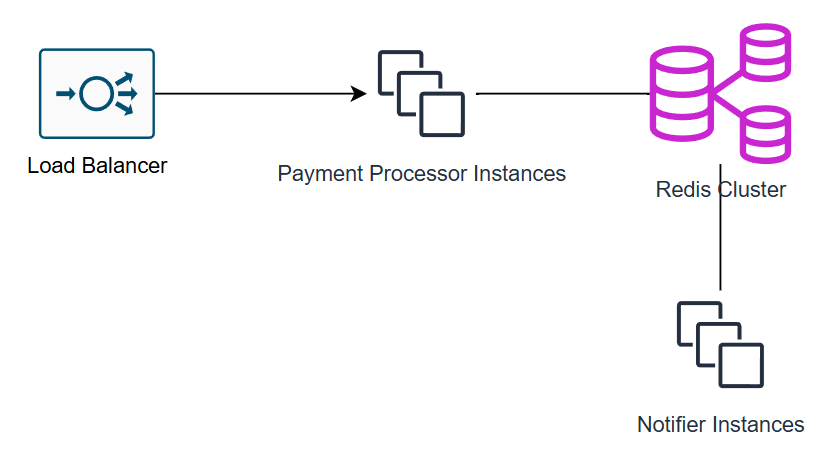
\includegraphics[width=0.65\textwidth]{resources/chapter-3/payment-service.png}
    \caption{Arsitektur Layanan Pembayaran}
    \label{fig:payment-service-deployment}
\end{figure}

\section{Alur Layanan}

Gambar \ref{fig:payment-flow1} menunjukkan alur sistem pembayaran untuk fitur pembuatan tagihan, pembayaran tagihan, dan baca data tagihan.

\begin{figure}[htbp]
    \centering
    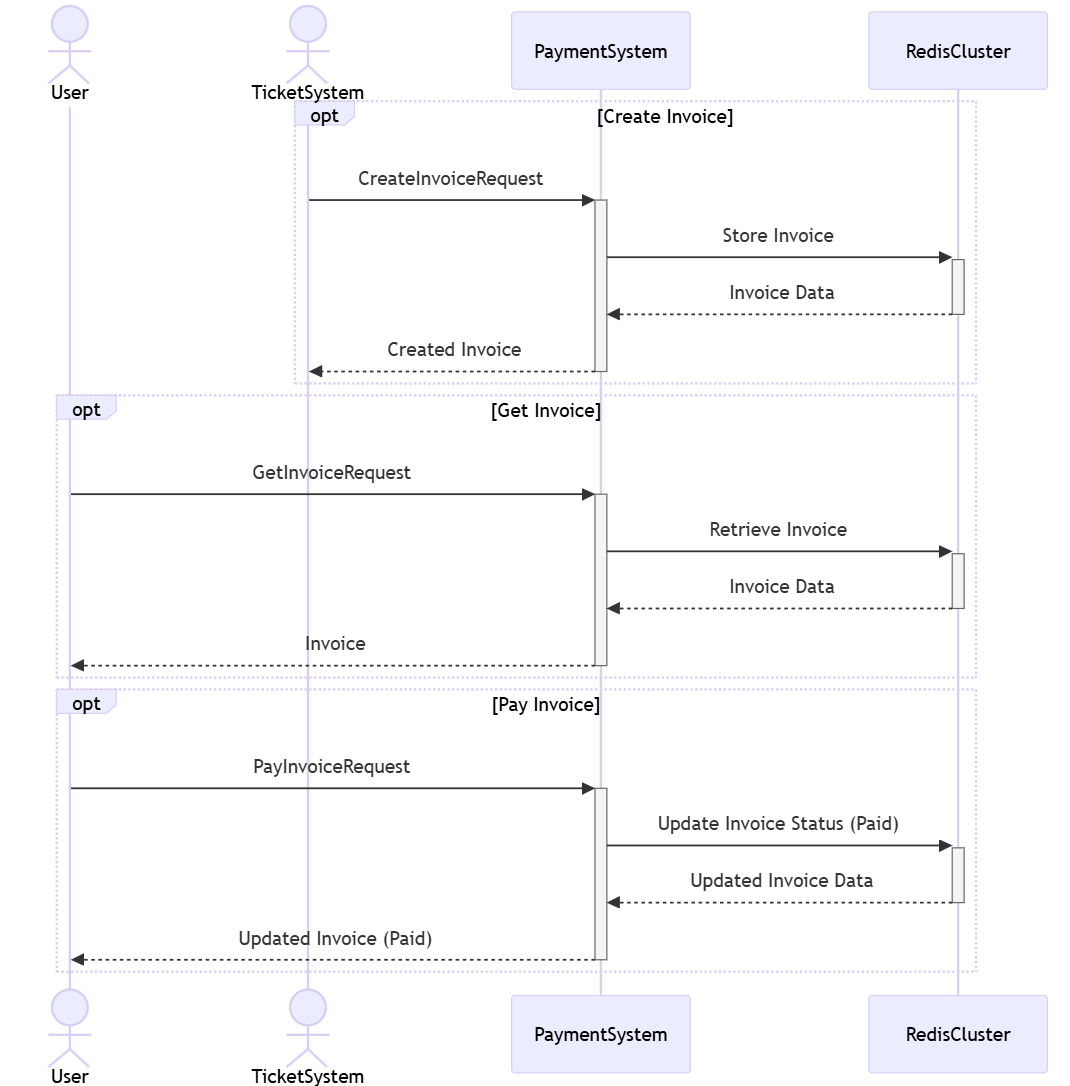
\includegraphics[width=0.75\textwidth]{resources/chapter-3/payment-flow1.png}
    \caption{Diagram Alur Pembuatan, Pembayaran dan Baca Tagihan}
    \label{fig:payment-flow1}
\end{figure}

\pagebreak

Selanjutnya, Gambar \ref{fig:payment-flow2} menunjukkan alur pemrosesan \textit{webhook} untuk pembayaran pemesanan yang berhasil atau pun gagal. Skema ini menggunakan strategi \textit{exponential backoff} untuk menangani kasus pemberitahuan yang gagal.

\begin{figure}[htbp]
    \centering
    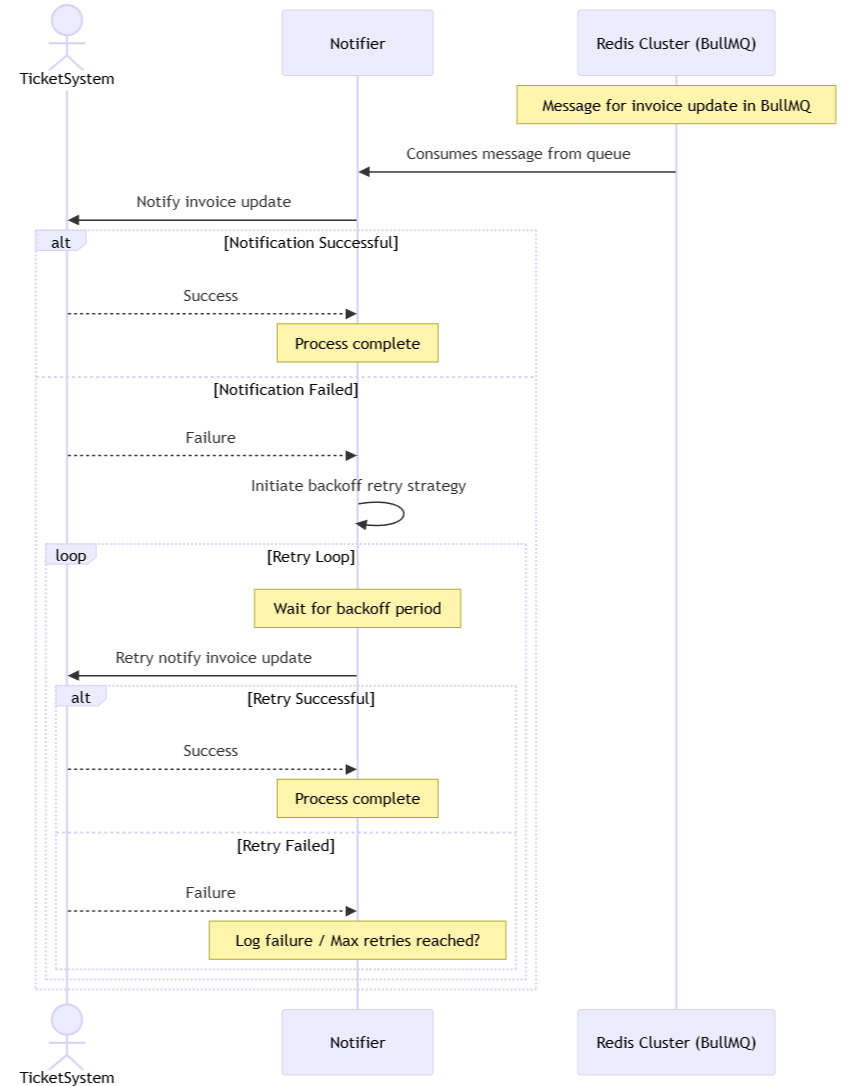
\includegraphics[width=0.8\textwidth]{resources/chapter-3/payment-flow2.png}
    \caption{Diagram Alur Pemrosesan \textit{Webhook}}
    \label{fig:payment-flow2}
\end{figure}